\documentclass[a4paper]{ctexart}
\usepackage{xeCJK}
\usepackage{times}
\usepackage{setspace}
\usepackage{fancyhdr}
\usepackage{graphicx}
\usepackage{wrapfig}
\usepackage{array}
\usepackage{fontspec,xunicode,xltxtra}
\usepackage{titlesec}
\usepackage{titletoc}
\usepackage[titletoc]{appendix}
\usepackage[top=30mm,bottom=30mm,left=20mm,right=20mm]{geometry}
\usepackage{enumerate}
\usepackage{caption}
\usepackage{abstract}
\usepackage{amsmath}
\usepackage{cite}
\setmainfont{TeX Gyre Pagella}

\captionsetup[figure]{name={图},labelsep=period,font={bf,small}}

%---------------------------------------------------------------------
%	页眉页脚设置
%---------------------------------------------------------------------
\fancypagestyle{plain}{\pagestyle{fancy}}%改变章节首页页眉
\pagestyle{fancy}
\lhead{\kaishu~视觉物联网课程作业~}
\rhead{\kaishu~1030616134~尹达恒}
\cfoot{\thepage}

%---------------------------------------------------------------------
%	目录页设置
%---------------------------------------------------------------------
\titlecontents{section}[2em]{\vspace{0.1\baselineskip}\songti\zihao{-4}}{\thecontentslabel\ }{}
{\hspace{.5em}\titlerule*[4pt]{$\cdot$}\contentspage}
\titlecontents{subsection}[4em]{\vspace{0.1\baselineskip}\songti\zihao{-4}}{\thecontentslabel\ }{}
{\hspace{.5em}\titlerule*[4pt]{$\cdot$}\contentspage}

\ctexset {
	section = {
		number = \arabic{section},
		format = \Large\bfseries,
	},
	subsection = {
		number = \arabic{section}.\arabic{subsection},
	}
}

\begin{document}
%---------------------------------------------------------------------
%	封面设置
%---------------------------------------------------------------------
\begin{titlepage}
	\begin{center}
    
\includegraphics[width=0.9\textwidth]{figure//Njust.png}\\
    \vspace{10mm}
    \textbf{\zihao{2}\kaishu{物联网工程学院}}\\[0.8cm]
    \textbf{\zihao{2}\kaishu{视觉物联网课程作业}}\\[3cm]
    \textbf{\zihao{2}\kaishu{基于颜色的图片人脸检测方法}}\\
    \textbf{\zihao{2}\kaishu{在不同颜色空间下的效果对比与分析}}\\[3cm]
	\vspace{\fill}
	\setlength{\extrarowheight}{3mm}
	{\songti\zihao{3}	
		\begin{tabular}{rl}
			{\makebox[4\ccwd][s]{班\qquad 级:}}& ~\kaishu 物联1601\\
			{\makebox[4\ccwd][s]{姓\qquad 名:}}& ~\kaishu 尹达恒 \\
			{\makebox[4\ccwd][s]{学\qquad 号:}}& ~\kaishu 1030616134\\
			{\makebox[4\ccwd][s]{指导老师:}} & ~\kaishu 陈莹\\
		\end{tabular}
	}\\[2cm]
	\vspace{\fill}
	\zihao{4}
	2018\textasciitilde 2019第二学期\\
	\today
	\end{center}	
\end{titlepage}



%---------------------------------------------------------------------
%  目录页
%---------------------------------------------------------------------
\tableofcontents % 生成目录
\newpage
%---------------------------------------------------------------------
%  实验一
%---------------------------------------------------------------------
\begin{spacing}{1.5}
\songti\zihao{-4}
\section{引言}
图像中的人脸是一副图像最典型的特征之一,人脸检测也是图像处理的重要环节。人脸具有显著的颜色特征,基于颜色范围的人脸检测算法具有算法简单高效的特点,在一些简单场景下能够方便快速地识别出人脸区域,进而为进一步的图像处理操作提供必要的信息\cite{RN46}。在基于颜色范围的人脸检测算法中,选择所使用的颜色空间是确定人脸颜色范围前的一个重要步骤,不同颜色空间中对同一颜色的描述向量各不相同,颜色的连续性和各种不同颜色之间的距离也有所差异\cite{RN48},因而在不同颜色空间中,基于颜色范围的人脸检测算法的检测效果也有较大差别。本文将简要介绍颜色空间理论和一些主流颜色空间的表示方法,并通过实际识别测试和对比分析探讨在各种颜色空间下基于颜色范围的人脸检测算法的可行性及有效性。
\section{原理与技术}
\subsection{颜色空间}
颜色空间是描述使用一组值(通常使用三个、四个值或者颜色成分)表示颜色方法的抽象数学模型。目前常见的颜色空间主要有以下几种:
\begin{enumerate}
	\item RGB:RGB颜色空间的编码方式和计算机色彩显示器显示色彩的原理相似,都是采用红(Red)、绿(Green)、蓝(Blue)相加混色的原理,通过指定三种颜色的成分值进而确定颜色\cite{RN47}。
	\item HSV:HSV是一种将RGB颜色空间中的点在倒圆锥体中的表示方法。HSV即色相(Hue)、饱和度(Saturation)、明度(Value),又称HSB(B即Brightness)。
	\item HSL:HSL代表色调(Hue),饱和度(Saturation)和亮度(Lightness),通常也称为HLS\cite{RN50}。
	\item YUV:YUV(亦称YCrCb)由亮度信号Y和两个色差信号R-Y(即U)、B-Y(即V)组成\cite{RN52}。
	\item CIE XYZ:CIE XYZ颜色空间就是在RGB系统的基础上,用数学方法,选用三个理想的原色来代替实际的三原色,从而将CIE-RGB系统中的光谱三刺激值和色度坐标r、g、b均变为正值。
	\item CIE Lab:Lab颜色空间由三个要素组成,一个要素是亮度(L),a 和b是两个颜色通道。a包括的颜色是从深绿色(低亮度值)到灰色(中亮度值)再到亮粉红色(高亮度值);b是从亮蓝色(低亮度值)到灰色(中亮度值)再到黄色(高亮度值)\citen{RN49}。
	\item CIE Luv:LUV颜色空间全称CIE 1976(L*,u*,v*)(也作CIE Luv)颜色空间,L*表示物体亮度,u*和v*是色度\cite{RN51}。
\end{enumerate}
本文将选用RGB和HSV两种颜色空间进行人脸检测算法对比。
\subsection{布尔掩膜}
掩膜又称掩像,是指用选定的图像、图形或物体,对处理的图像(全部或局部)进行遮挡,来控制图像处理的区域或处理过程,是一种重要的图像区域提取方法\cite{RN53}。其中布尔掩膜是用预先制作的感兴趣区0-1矩阵与待处理图像按位相乘,得到感兴趣区图像,使感兴趣区内图像值保持不变,而区外图像值都为0,以达到图像区域提取的目的。以RGB空间为例,布尔掩膜在RGB图片的表达式如下:
\begin{equation}
\label{eq1}
\begin{split}
P^{*}(X)=&P(X)\cdot M\\
X\in&\{R,G,B\}\\
\end{split}
\end{equation}
其中$P$表示原始图像,$M$表示一个0-1矩阵,$P^{*}$表示经过布尔掩膜后的图像,$P(X)$和$P^{*}(X)$分别表示掩膜前后图像的$X$颜色分量矩阵。
\section{实验步骤}
\subsection{数据收集}
本文的训练图片和测试图片均来源与百度图片中搜索“人脸”关键词所得网络图像。为方便取色,训练图片集的选择标准为光照良好,人脸清晰,且背景单一的人脸图片;测试图片集选择光照良好,人脸清晰,背景非统一色块的人脸图片。图片量为训练图片4张,测试图片2张。
\subsection{确定人脸颜色范围}
\subsubsection{取样}
确定颜色范围时需要在训练图片中指定区域位置和取样方法。为保证统计的准确性,本文先从每张图片的人物脸部明亮部分和阴影部分各选出一个$100\times100$共10000像素的区域,通过4张训练图片共计8个取样区域内的像素确定人脸的颜色范围。各图像的取样区域和取样结果见图\ref{spa}和图\ref{sp}。

\begin{figure}[htbp]
	\centering
	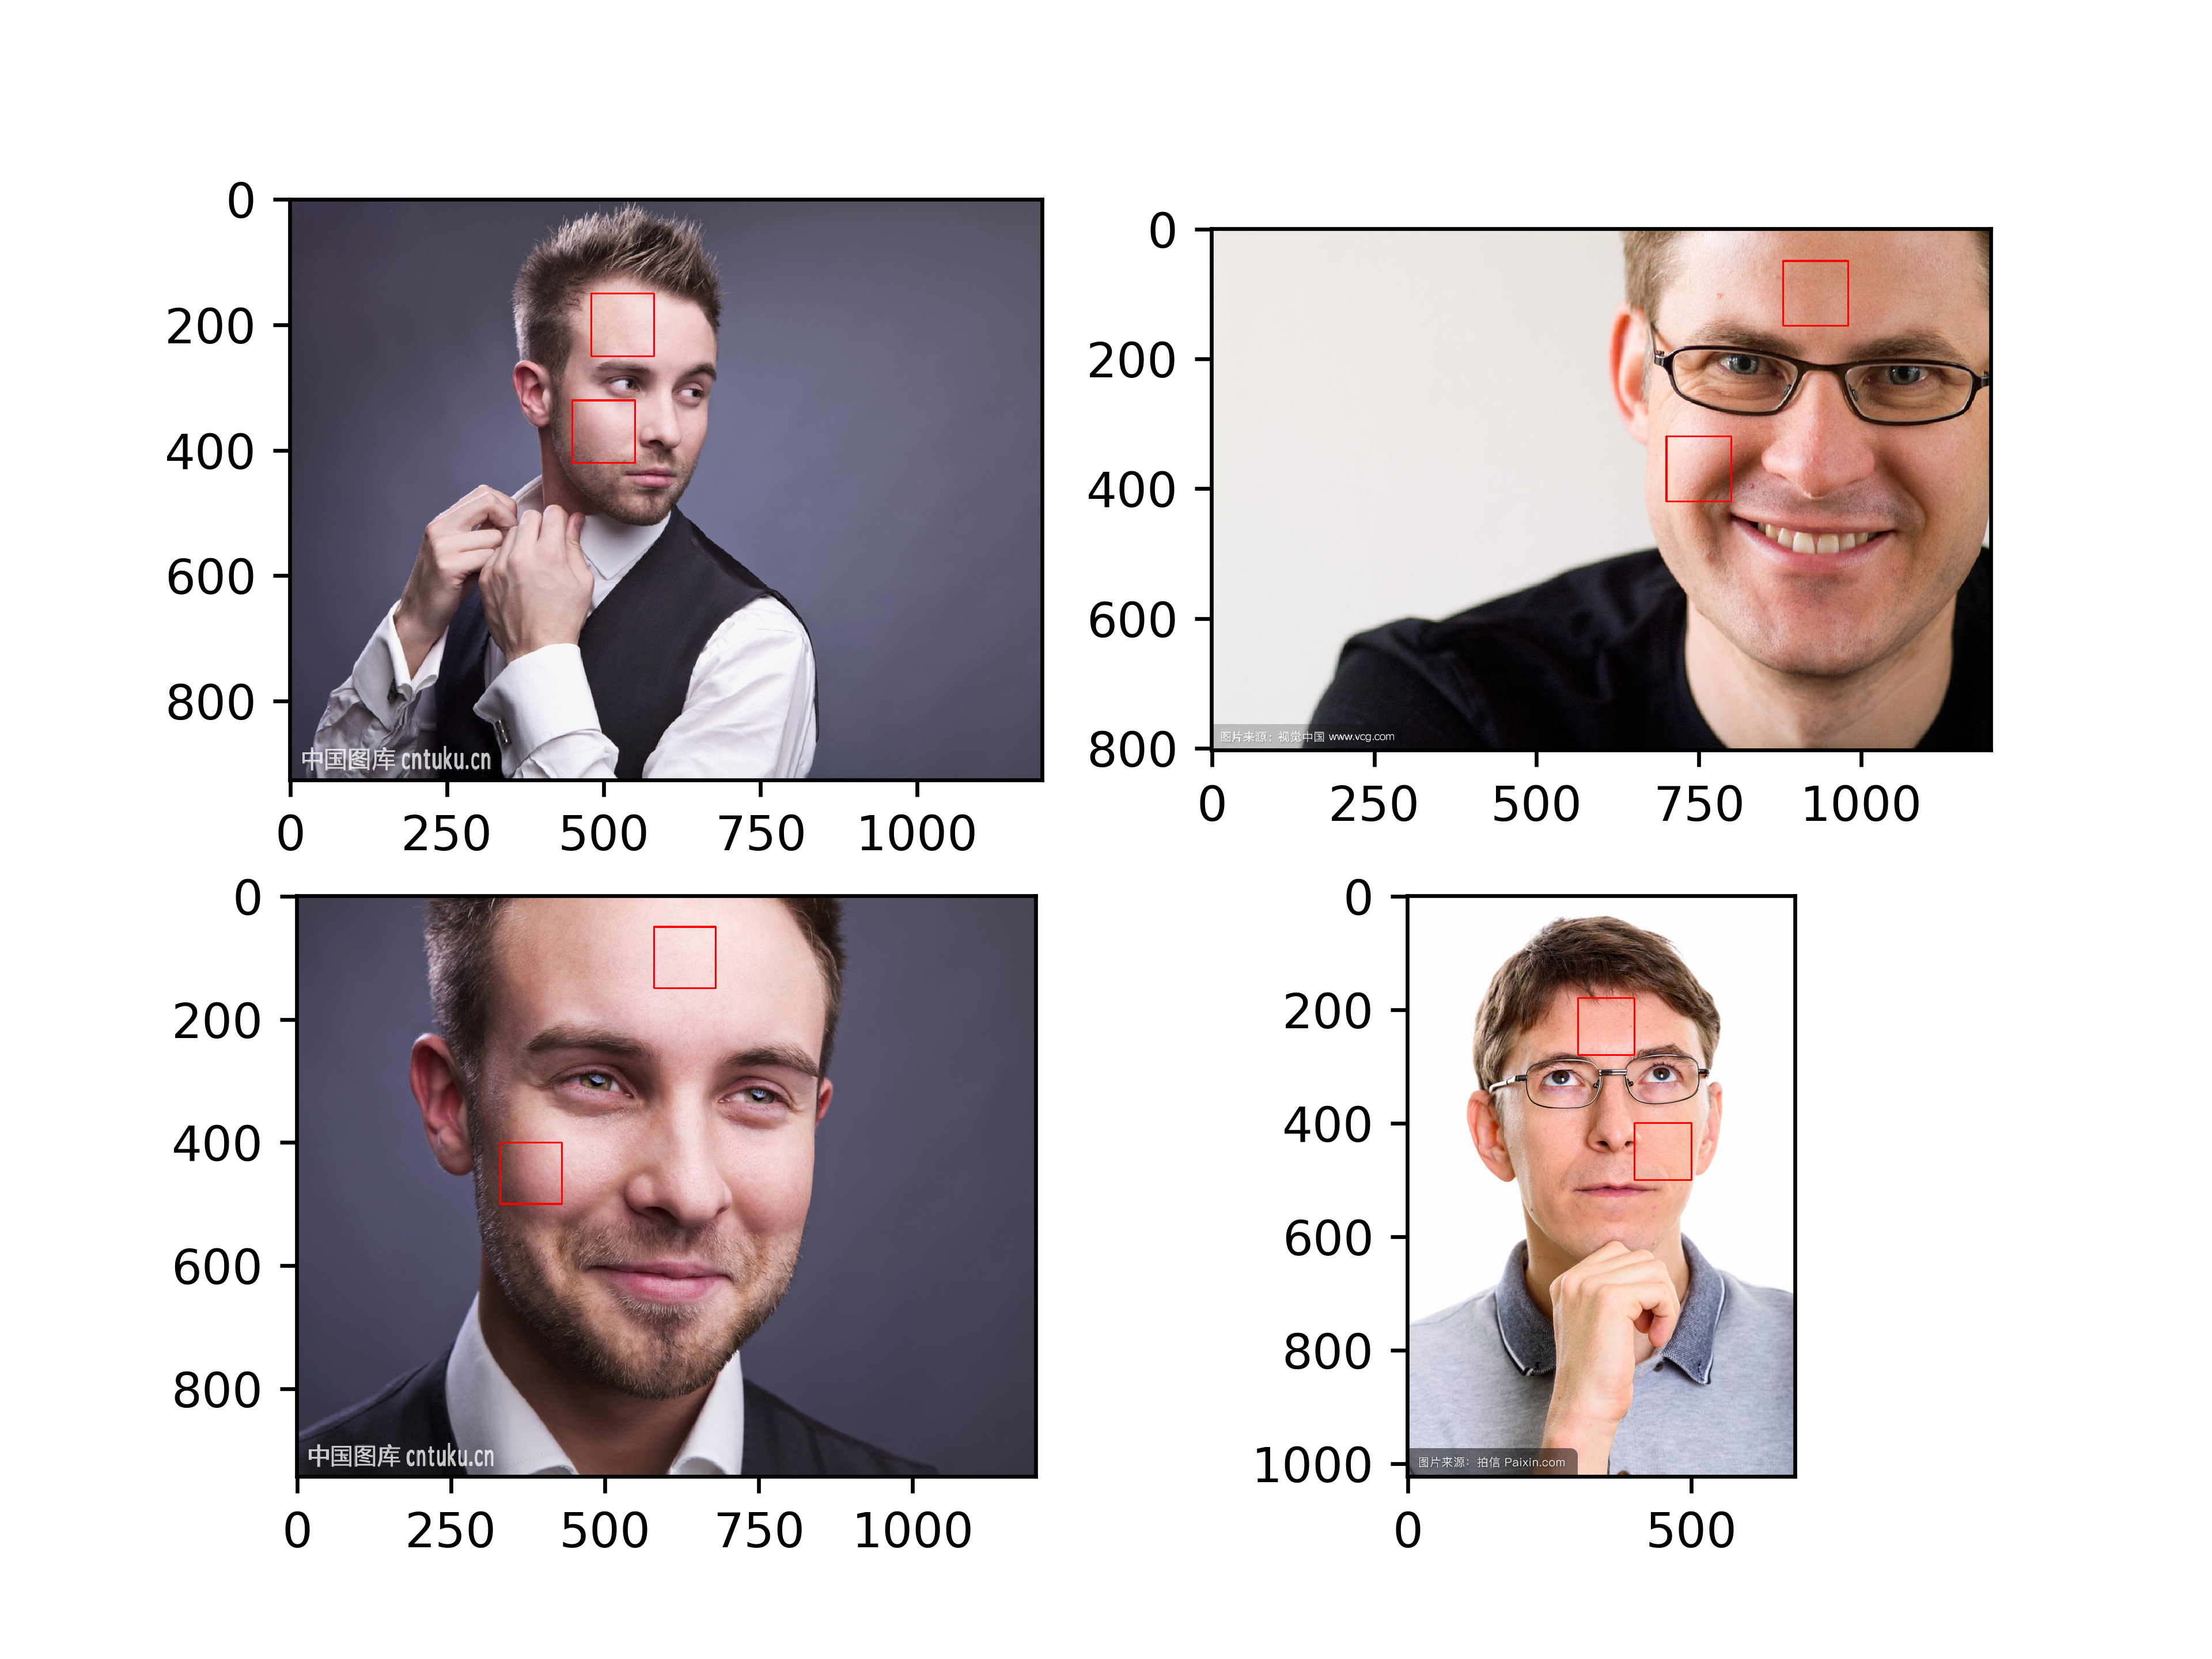
\includegraphics [width=0.8\textwidth]{figure//spa.png}
	\caption{取样区域(红色方框)}\label{spa}
\end{figure}
\begin{figure}[htbp]
	\centering
	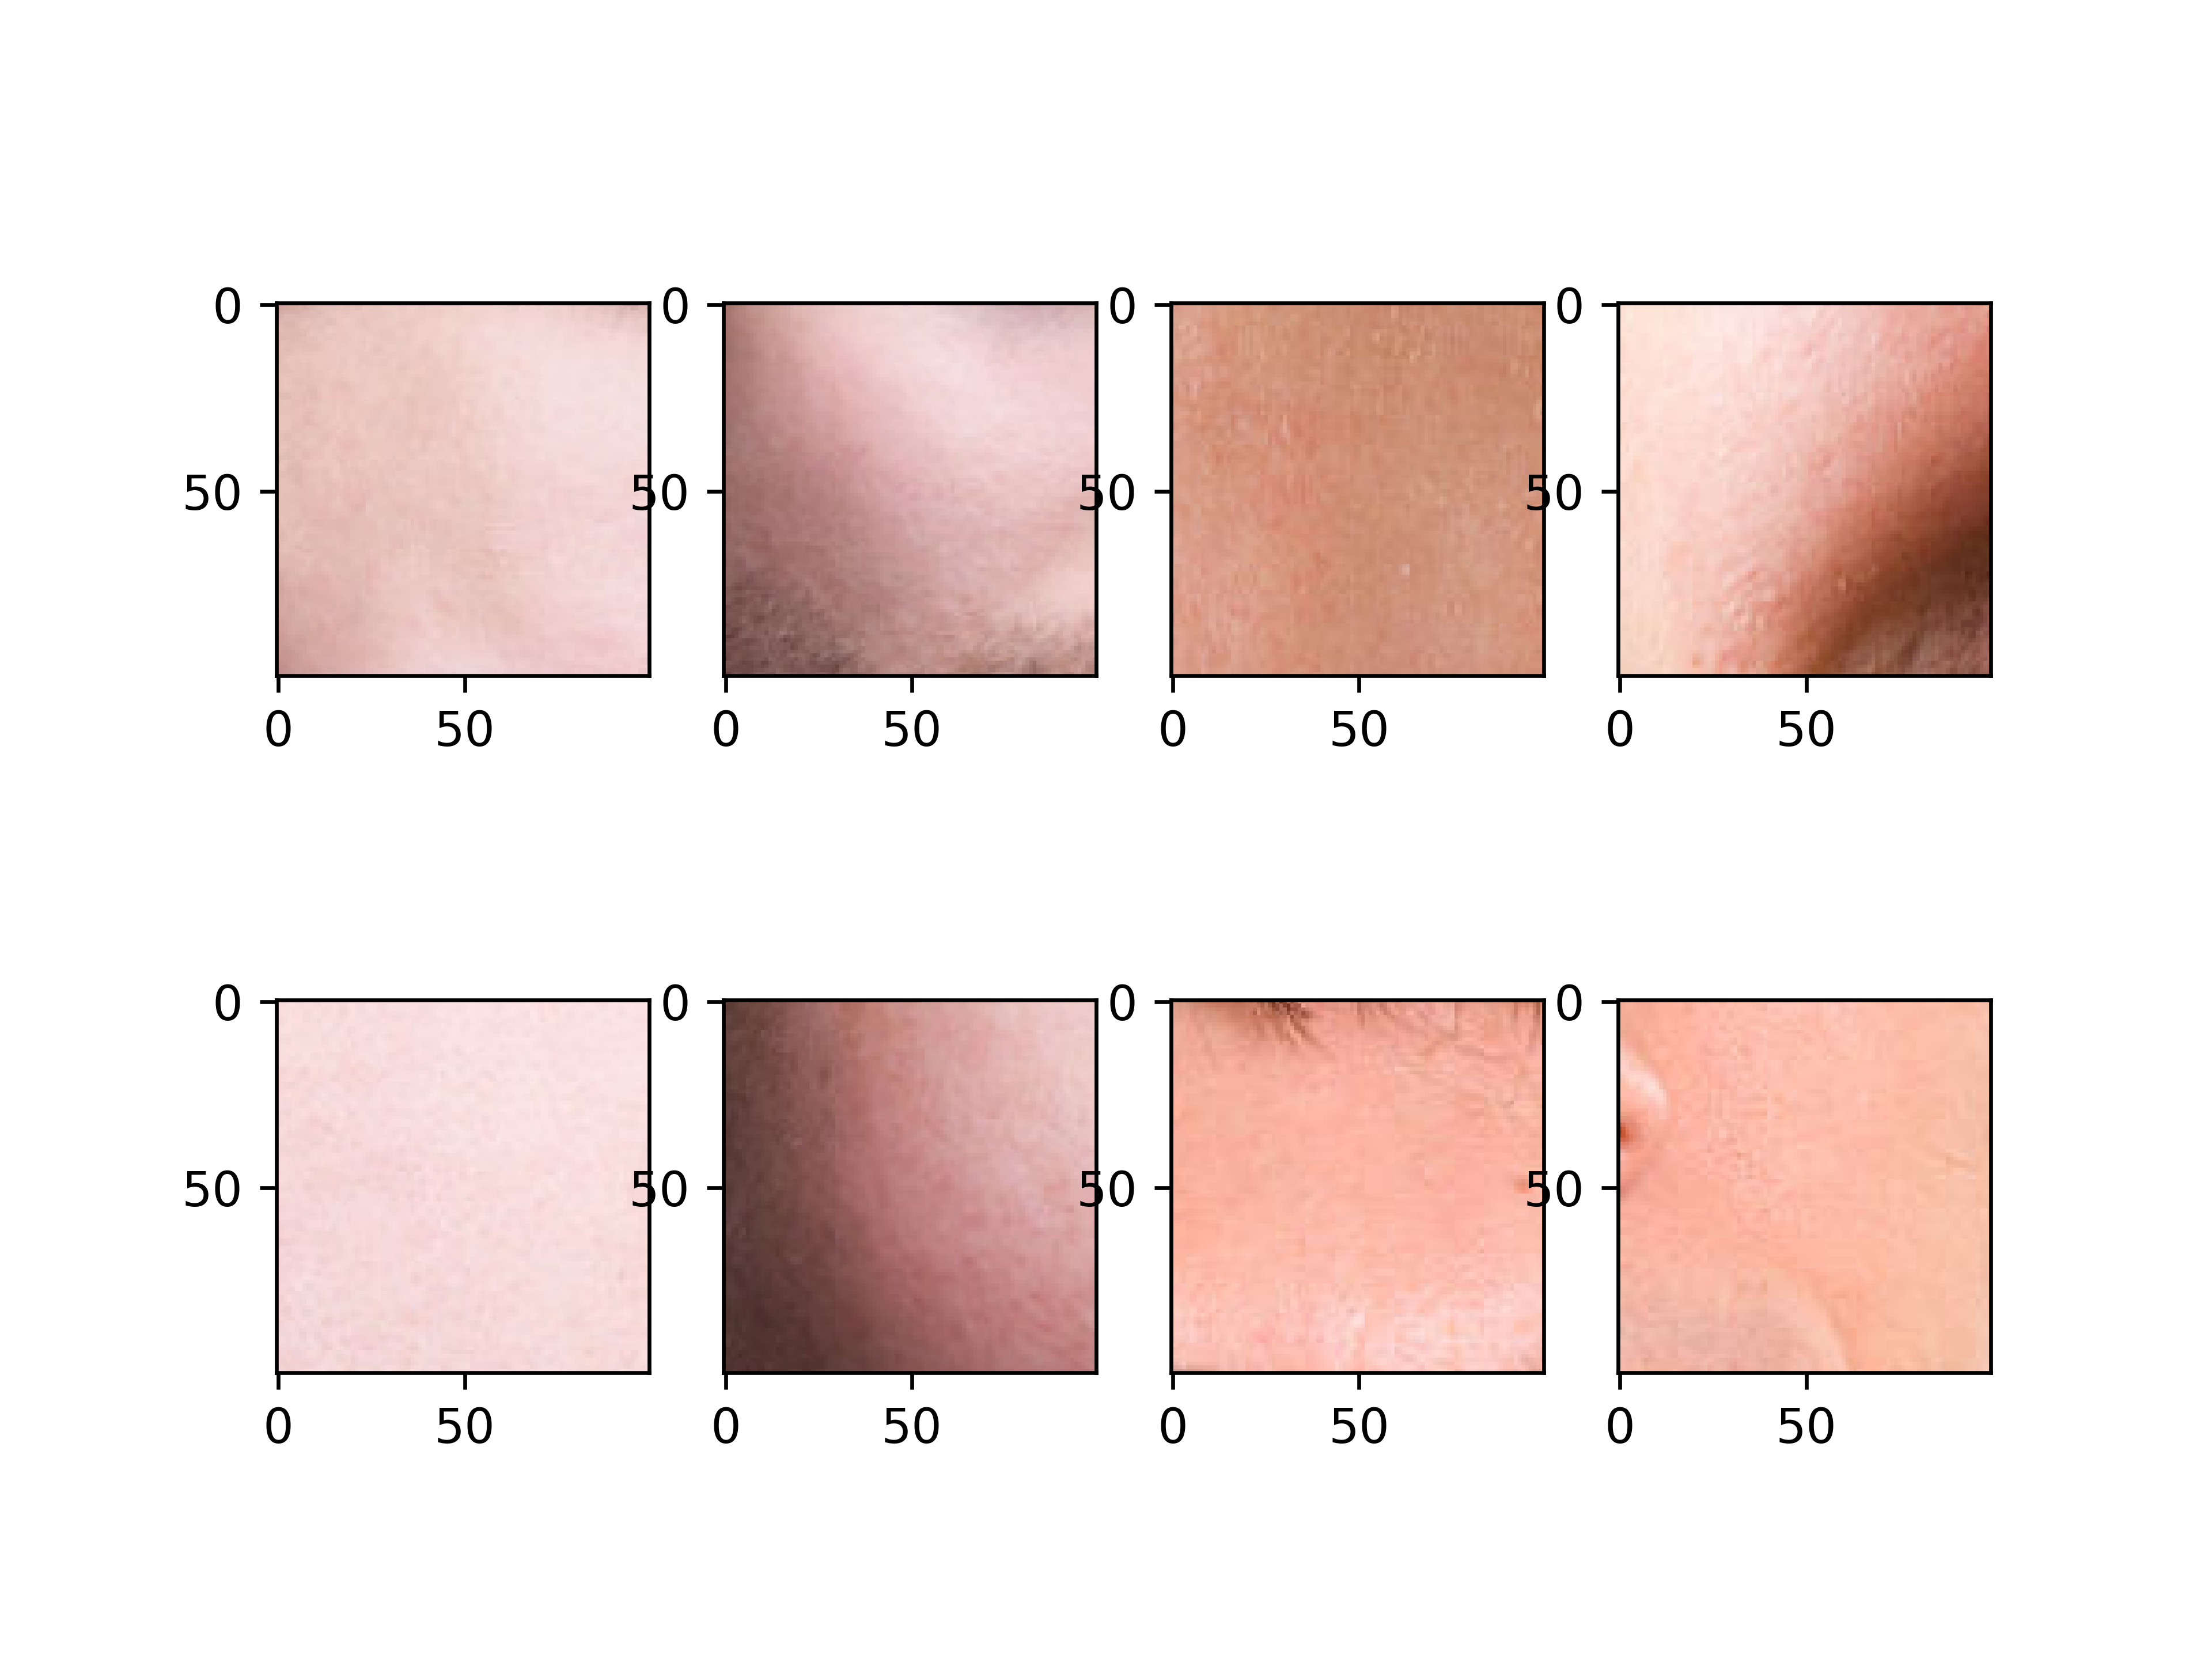
\includegraphics [width=0.8\textwidth]{figure//sp.png}
	\caption{取样结果}\label{sp}
\end{figure}
\subsubsection{统计}
在得到区域区域的数据之后,接下来便要通过区域区域各像素的颜色分量分布情况确定最佳的颜色范围。本文所用的方法是在获得样本区域所有像素点后,对不同颜色分量分别确定范围。以RGB颜色空间为例,具体步骤如下:
\begin{enumerate}
	\item 将图片的各颜色分量压缩为0\~255之间的整数,其中第$i$个像素的第$X$分量的值记作$p_{i,X},X\in\{R,G,B\}$;
	\item 分别统计每个颜色分量$X$中每个数值$p$出现的次数$N_{p,X}$;
	\item 分别对每个颜色分量$X$中每个数值$p$按照$N_{p,X}$的大小进行排名,找出每个颜色分量$X$中$N_{p,X}$最大的100个$p$值组成集合$P_{X},X\in\{R,G,B\}$;
	\item 计算每个颜色分量$X$的范围上界$p_{max}(X)=max(P_{X})$和下界$p_{min}(X)=min(P_{X})$。
\end{enumerate}
\subsection{检测人脸区域}
检测人脸区域实际上是求布尔掩膜中0-1矩阵$M$的过程,如果某个像素的颜色分量取值都落在对应的颜色分量范围内,则矩阵$M$对应位置的值为1,否则为0。以RGB颜色空间为例,其0-1矩阵$M$的表达式如下:
\begin{equation}
\begin{split}
M=&(m_{i,j})\\
m_{i,j}=&
\left\{
\begin{aligned}
1& &(\forall X\in\{R,G,B\},p_{min}(X)\leq p_{i,j}(X)\leq p_{max}(X))\\
0& &else\\
\end{aligned}
\right.
\end{split}
\end{equation}
其中$p_{i,j}(X)$为图像中像素$(i,j)$的$X$颜色分量的值。
\subsection{提取人脸区域}
提取人脸区域的过程实际上是通过式\ref{eq1}求掩膜后图像的过程。一个理想的人脸检测程序得出的掩膜图像应该能够包含全部的人脸区域且不包含人脸以外的区域。
\section{实验结果}
\begin{enumerate}
	\item 每个颜色分量$X$中每个数值$p$出现的次数$N_{p,X}$如图\ref{reslin}所示;
	\item 在RGB和HSV颜色空间内的掩膜结果如图\ref{respic}所示;
\end{enumerate}
\begin{figure}[htbp]
	\centering
	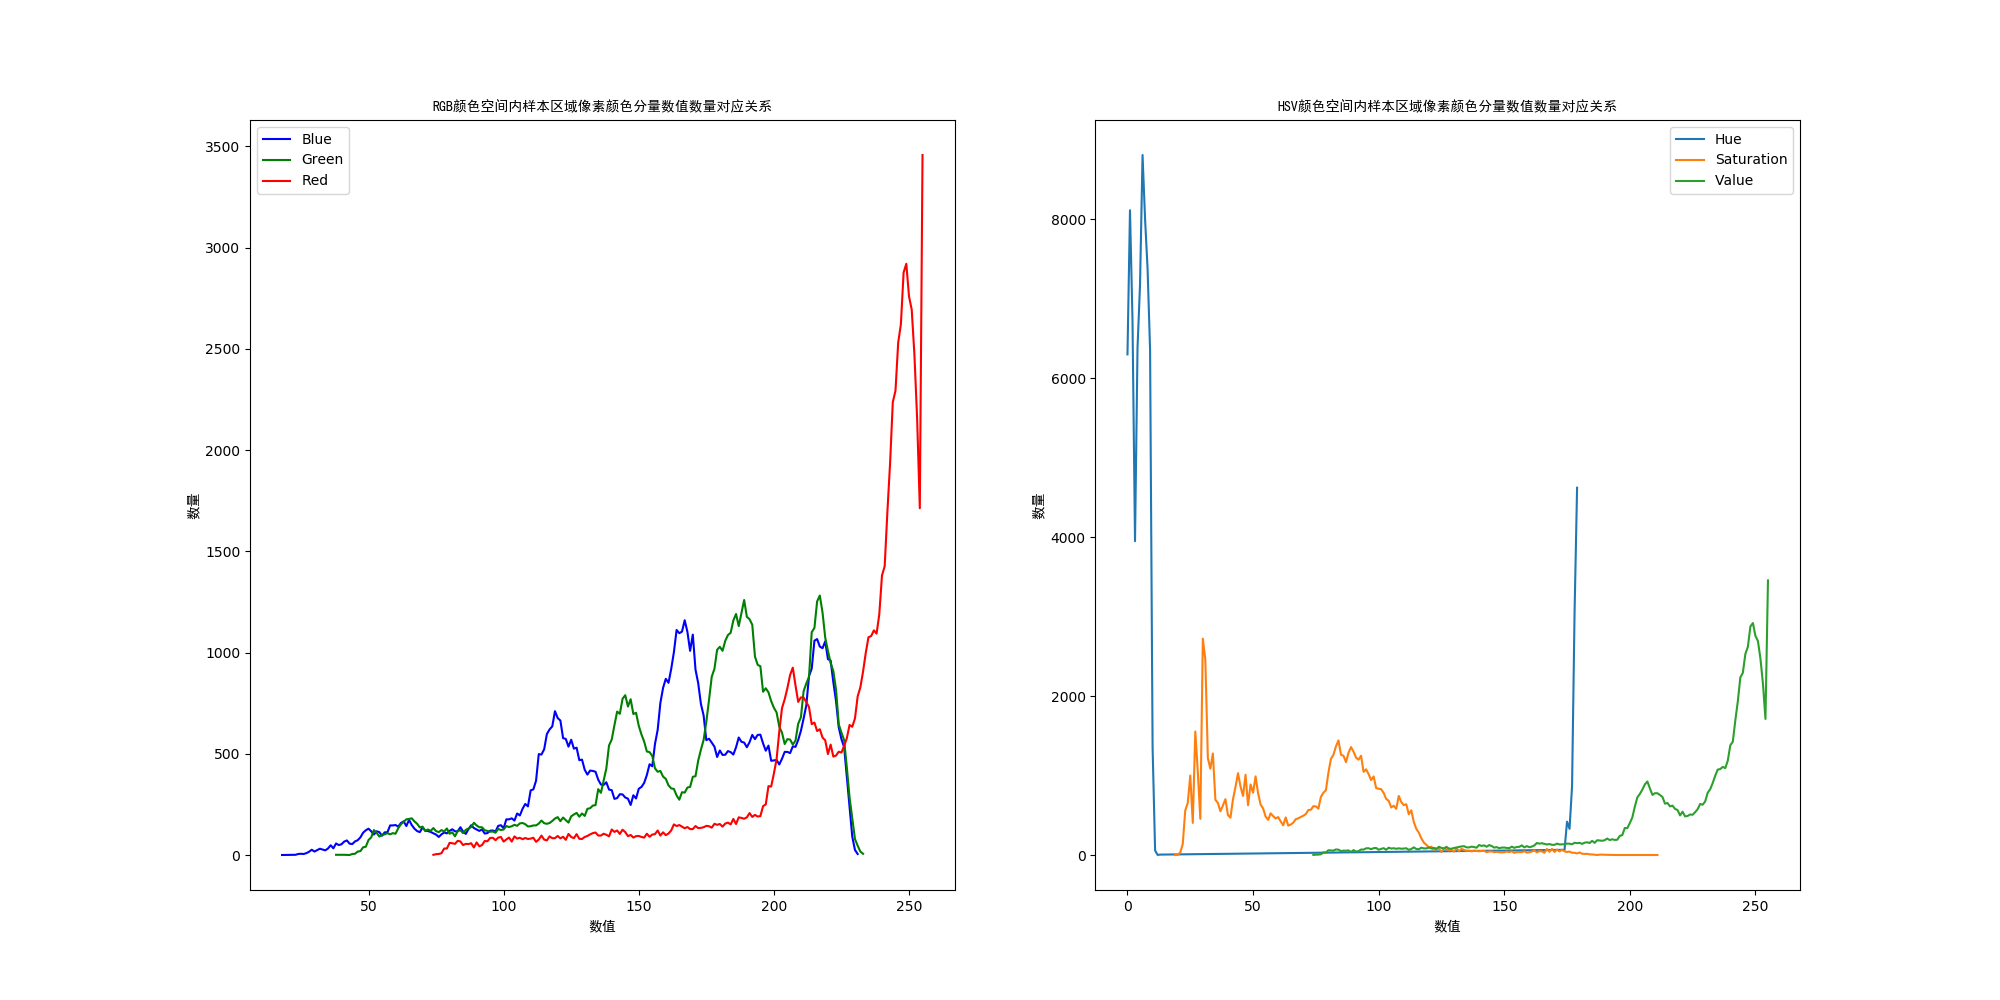
\includegraphics [width=0.8\textwidth]{figure//res2.png}
	\caption{取样统计结果}\label{reslin}
\end{figure}
\begin{figure}[htbp]
\centering
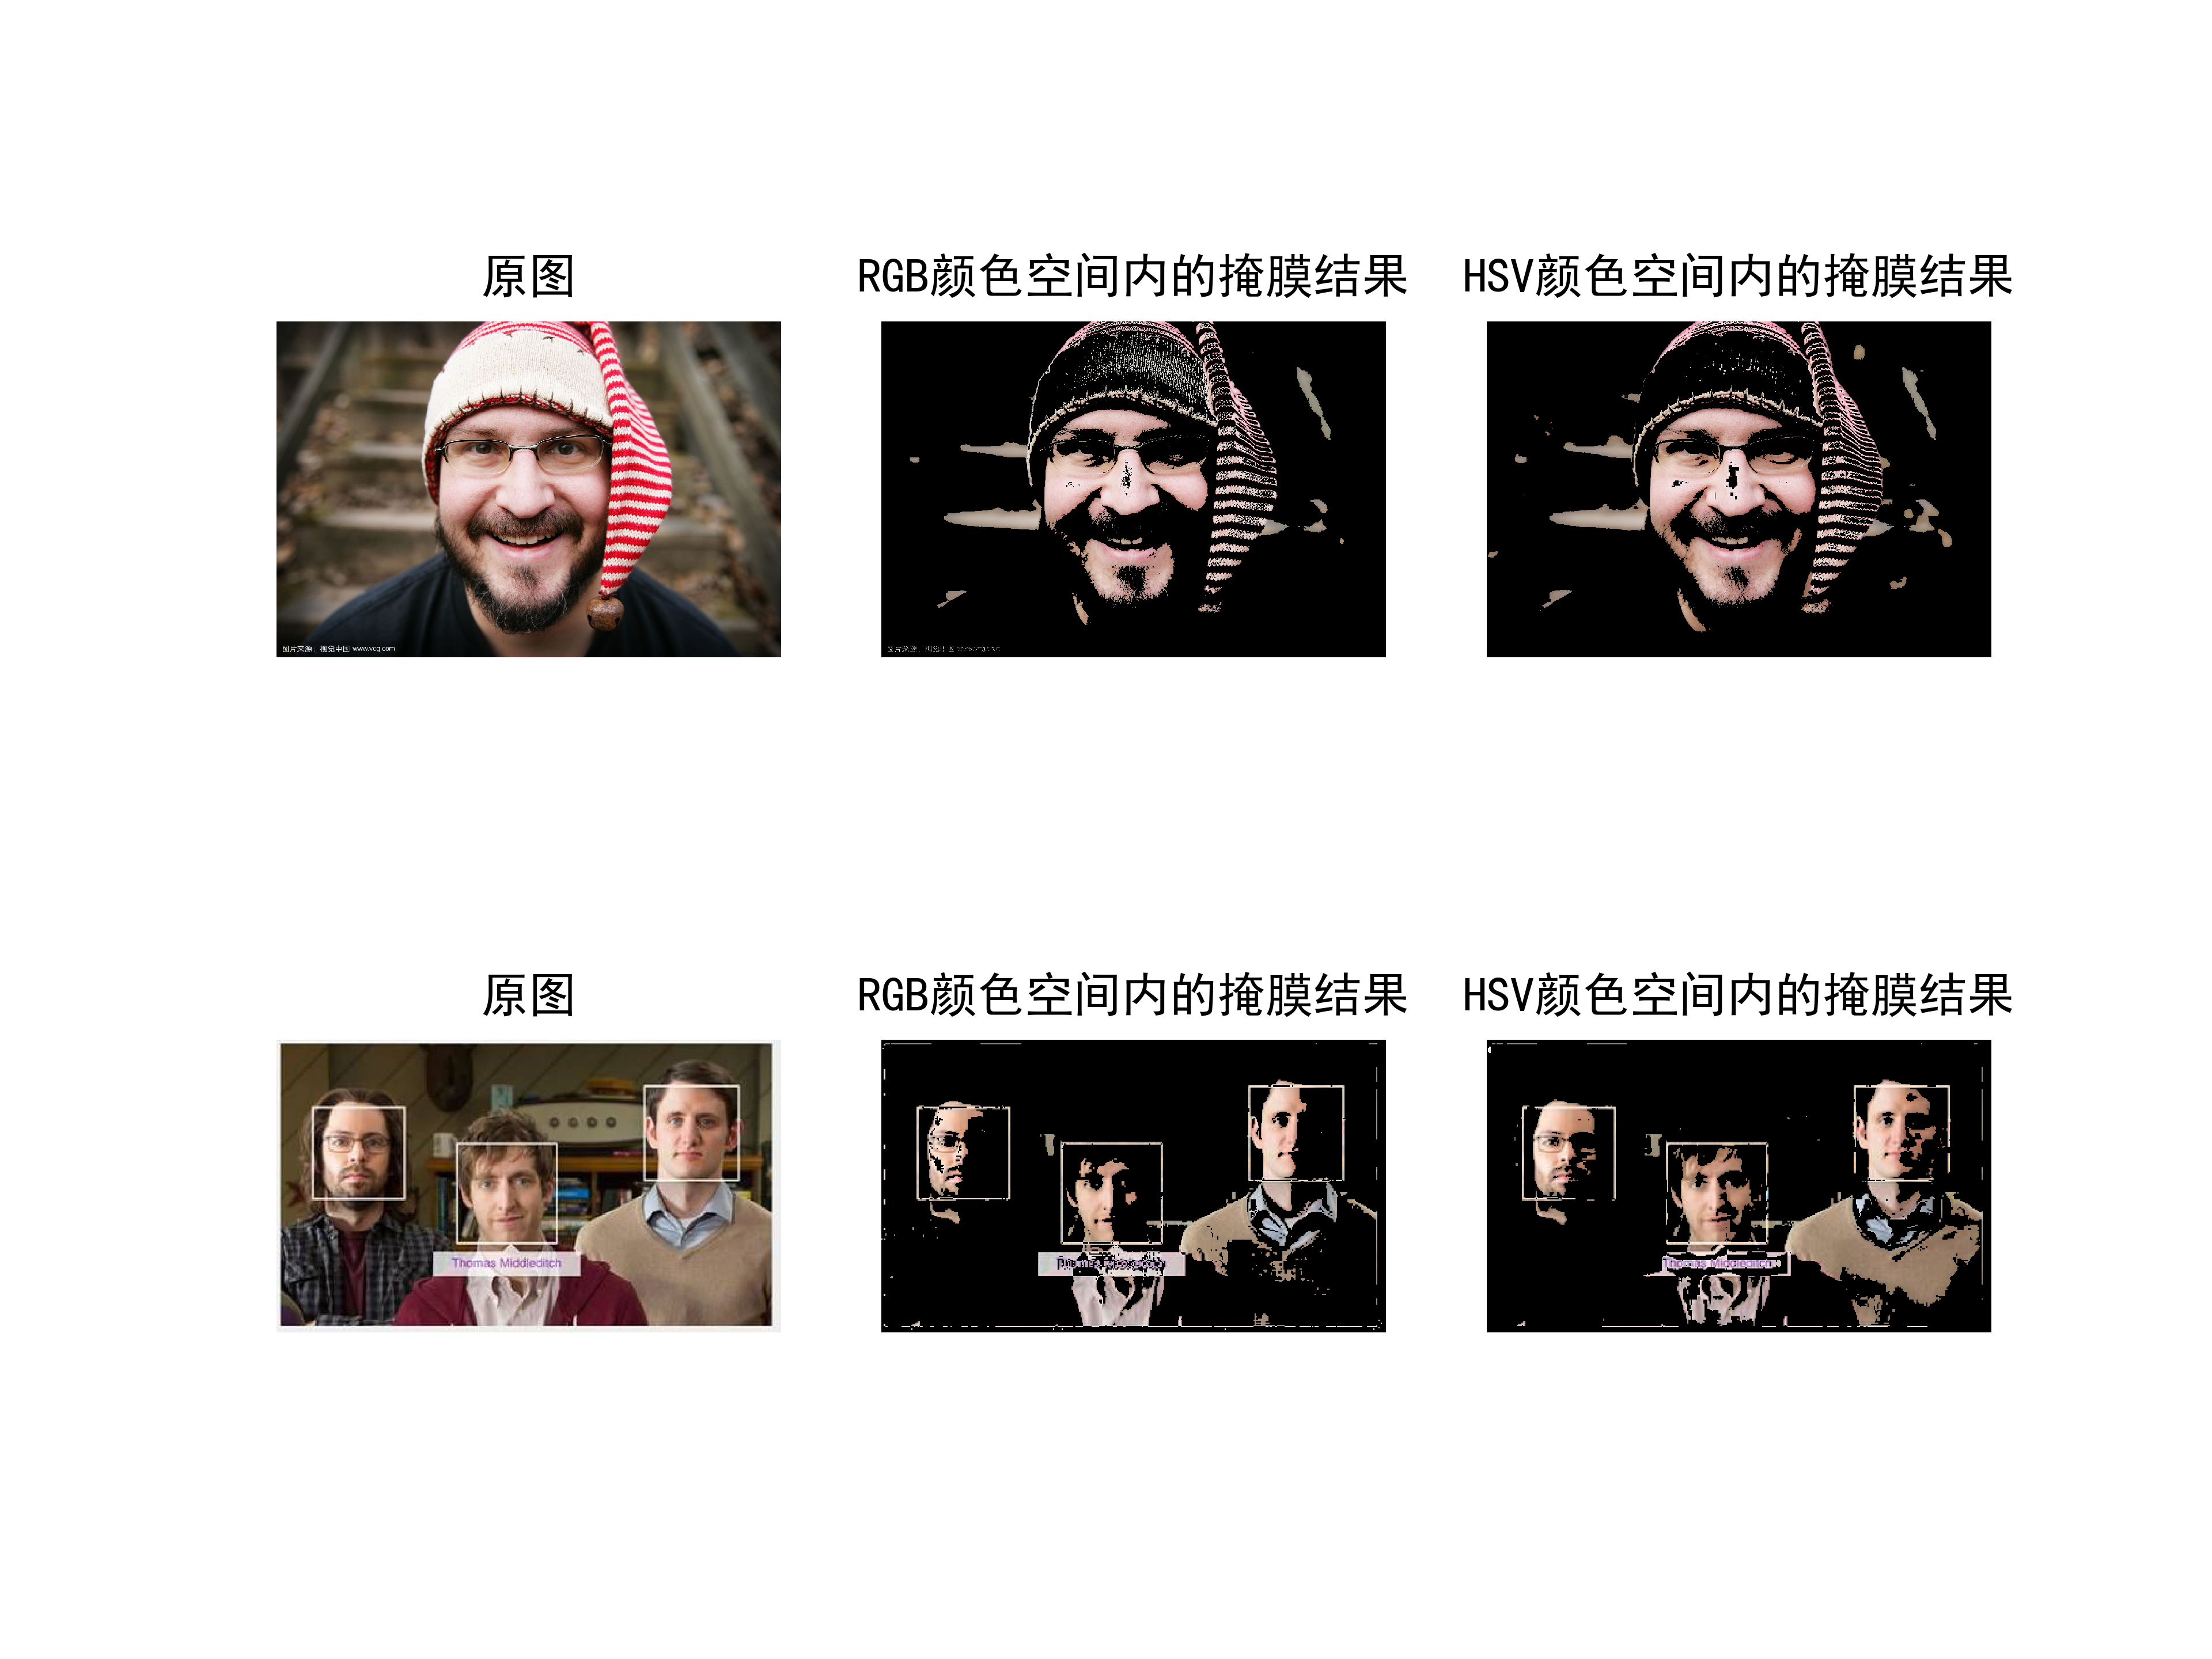
\includegraphics [width=0.8\textwidth]{figure//res1.png}
\caption{掩膜结果}\label{respic}
\end{figure}
从图\ref{respic}中可以看出,RGB色彩空间内的各种颜色分量数值的数量具有明显的波动性,表明在RGB颜色空间内,相近的颜色在空间内的距离不一定接近;而HSV颜色空间内的颜色分布趋于集中,表明相近的颜色在HSV颜色空间内的距离比在RGB颜色空间内的距离更加接近。从图\ref{respic}中可以看出,相较于RGB颜色空间,在HSV颜色空间内进行的掩膜所覆盖的人脸区域更多,非人脸区域更少。
\section{结论}
RGB颜色空间的色彩分布规律不利于基于颜色的检测算法。在HSV颜色空间内进行基于颜色的人脸检测要比在RGB颜色空间内有更好的效果。
\end{spacing}
\bibliography{ref}
\bibliographystyle{unsrt}
\end{document}